\chapter{\IfLanguageName{dutch}{Proof of concept}{Proof of concept}}%
\label{ch:proof-of-concept}

\section{Proof of Concept: Real-time Monitoring via Centrale en Edge Databases}

Deze proof of concept heeft als doel het prestatieverschil te analyseren tussen twee implementaties voor real-time monitoring: een traditionele centrale database-architectuur (Gebouw A) en een edge computing-architectuur met lokale verwerking (Gebouw B). De focus ligt op typische IoT-sensordata zoals \ce{CO2}-metingen, temperatuur en luchtdruk.

Beide scenario's worden opgezet met Docker Compose om gescheiden en reproduceerbare testomgevingen te garanderen. Binnen elk scenario worden verschillende databases getest met meerdere datapartitioneringstechnieken (zoals range-based en list-based partitionering) om te bepalen welke het meest geschikt is voor centrale versus gedistribueerde verwerking.
\section{Functionele en niet-functionele Eisen}

\subsection{Functionele eisen}

De functionele eisen beschrijven wat het systeem concreet moet doen. Voor deze proof of concept binnen de HoGent-use case werden volgende functionele eisen gedefinieerd:

\begin{itemize}
    \item Het systeem moet om de 5 seconden de waarden van \ce{CO2}, temperatuur en luchtdruk registreren.
    \item Het systeem moet een waarschuwing tonen wanneer de \ce{CO2}-waarde de drempel van 800 ppm overschrijdt.
    \item Het systeem moet real-time grafieken tonen met de evolutie van de \ce{CO2}-waarden.
    \item Het systeem moet historische meetgegevens kunnen opvragen per lokaal.
    \item Het systeem moet logs bijhouden van wanneer drempelwaarden zijn overschreden.
    \item Het systeem moet foutmeldingen tonen bij verbindingsproblemen met de database of edge-node.
\end{itemize}

\subsection{Niet-functionele eisen}

Niet-functionele eisen beschrijven de kwaliteitseigenschappen van het systeem. Dit zijn de niet-functionele eisen voor het systeem:

\begin{itemize}
    \item \textbf{Performantie:} Het systeem moet lage latentie hebben ($<$ 500 ms) bij het tonen van nieuwe meetdata.
    \item \textbf{Schaalbaarheid:} Het systeem moet uitbreidbaar zijn naar meerdere lokalen zonder herconfiguratie. Ook horizontale schaalbaarheid over meerdere nodes moet ondersteund worden zonder prestatiedaling.
    \item \textbf{Fouttolerantie:} Het systeem moet blijven functioneren bij netwerkstoringen of node-uitval, zonder dataverlies.
    \item \textbf{Offline werking en synchronisatie:} Het systeem moet tijdelijk lokaal data kunnen opslaan en veilig synchroniseren zodra netwerkverbinding is hersteld.
    \item \textbf{Lokale verwerking:} De edge-node moet in staat zijn om data lokaal te verwerken om latentie en netwerkbelasting te minimaliseren.
    \item \textbf{Geheugengebruik en CPU-belasting:} De database moet efficiënt werken op edge-devices met beperkte hardwarecapaciteit.
    \item \textbf{Doorvoersnelheid:} Het systeem moet hoge frequenties van sensordata kunnen verwerken (inserts per seconde).
    \item \textbf{Gegevensconsistentie:} Alle nodes moeten beschikken over een betrouwbare en gelijke data.
    \item \textbf{Beheer en onderhoud:} De configuratie, monitoring en foutafhandeling van het systeem moeten eenvoudig zijn.
    %\item \textbf{Gebruiksvriendelijkheid:} De gebruikersinterface moet duidelijk en eenvoudig te gebruiken zijn.
    \item \textbf{Beveiliging:} Data moet veilig worden opgeslagen en enkel toegankelijk zijn voor bevoegde gebruikers.
    %\item \textbf{Beheerbaarheid:} Het systeem moet eenvoudig instelbaar zijn via een \texttt{.env}-bestand of dashboard.
\end{itemize}

\section{Architectuurscenario's per gebouw}
\subsection{Gebouw A - Centrale Database Architectuur}

Gebouw A maakt gebruik van een traditionele architectuur waarin alle meetgegevens van de sensoren in de lokalen (zoals A101, A102, A103) via het netwerk worden doorgestuurd naar een centrale server. Deze server bevat een relationele database waarin alle data centraal wordt opgeslagen.

\subsection{Gebouw B - Edge Computing Architectuur}

Gebouw B is uitgerust met een edge computing-opzet waarbij elk lokaal (zoals B101, B102, B103) beschikt over een eigen edge-node. Deze node bevat een lokale database waarin meetgegevens direct worden opgeslagen en verwerkt. Drempelwaarde-evaluatie (bijvoorbeeld \ce{CO2} > 800 ppm) gebeurt lokaal, zonder dat een centrale server nodig is voor de initiële verwerking.

\subsection{Testdoelen in beide gebouwen:}
\begin{itemize}
    \item Verzamelen en opslaan van meetgegevens vanuit meerdere lokalen.
    \item Detectie van drempelwaarden (\ce{CO2} > 800 ppm) en genereren van waarschuwingen.
    \item Logging van drempeloverschrijdingen en opvraging van historische data.
    \item Evaluatie van systeemprestaties bij verhoogde belasting.
    \item Analyse van schaalbaarheid en gedrag bij uitbreiding naar meerdere lokalen.
    \item Meting van latency en doorvoersnelheid.
    \item Fouttolerantie en gedrag bij netwerkstoringen of node-uitval.
    \item Monitoring van resourcegebruik (CPU, geheugen).
\end{itemize}

\section{Ontwikkeling van de Applicatie}

De proof of concept is gerealiseerd met Docker Compose en gesimuleerde sensordata. De werking van de applicatie wordt getest aan de hand van concrete functionele eisen zoals het genereren van een waarschuwing wanneer het \ce{CO2}-gehalte hoger is dan 800 ppm.

\subsection{Architectuur}

De applicatie is opgebouwd als een real-time monitoringdashboard in een edge-omgeving met volgende componenten:

\begin{itemize}
    \item \textbf{IoT-sensor (gesimuleerd):} Genereert elke 5 seconden meetgegevens.
    \item \textbf{Edge-node:} Verwerkt en slaat lokaal data op met een te testen database-engine.
    \item \textbf{Backend (ASP.NET Core):} Verwerkt sensordata, detecteert overschrijding van drempelwaarden en verstuurt meldingen.
    \item \textbf{Frontend (React):} Visualiseert live-data en historische grafieken.
    \item \textbf{Docker Compose:} Beheert de opstelling van verschillende databases, backend en frontend in afzonderlijke containers.
\end{itemize}

\subsection{Melding bij \ce{CO2}-overschrijding}

Bij overschrijding van 800 ppm \ce{CO2}:
\begin{itemize}
    \item Wordt een rode waarschuwing getoond op het dashboard.
    \item Wordt een log-item toegevoegd aan de database.
    %\item (Optioneel) Wordt een melding verstuurd via e-mail of webhook.
\end{itemize}

\section{Tabellen en Datastructuren}

De gebruikte tabel heet \texttt{sensor\_data} en heeft een consistente structuur in alle databases.

\paragraph{Velden in \texttt{sensor\_data}:}
\begin{itemize}
    \item \texttt{sensor\_id (UUID)} - Unieke identificatie per sensor.
    \item \texttt{timestamp (TIMESTAMP)} - Tijdstip van de meting.
    \item \texttt{temperature (DOUBLE)} - Temperatuurwaarde.
    \item \texttt{co2 (INTEGER)} - CO₂-waarde in ppm.
    \item \texttt{pressure (DOUBLE)} - Luchtdruk in hPa.
    \item \texttt{status (TEXT)} - Sensorstatus ('actief', 'offline').
\end{itemize}

\paragraph{Toepassing per architectuur:}
\begin{itemize}
    \item \textbf{Gebouw A (centraal):} verschillende databases worden getest als centrale opslagoptie voor data uit alle lokalen.

    \item \textbf{Gebouw B (edge):} elk lokaal heeft een eigen edge-node waarop verschillende edge-geschikte databases worden getest.
\end{itemize}

\section{Workload Simulatie}

\paragraph{Datageneratie}
De \texttt{Faker.js}-bibliotheek wordt gebruikt om gesimuleerde sensorgegevens aan te maken, waaronder temperatuur, druk en \ce{CO2}-waarden. Er wordt bewust data gegenereerd met waarden boven 800 ppm om het waarschuwingssysteem te activeren.

\paragraph{Data-invoer}
Via Node.js-scripts wordt data naar de databases geschreven. Elke container ontvangt data alsof die afkomstig is uit een lokaal.

Elke test wordt herhaald voor verschillende database-engines in zowel Gebouw A als Gebouw B. Zo kan geëvalueerd worden welke database het best presteert binnen het gekozen architecturale model.

\paragraph{Functionele tests}
In beide gebouwen worden dezelfde functionele eisen getest:
\begin{itemize}
    \item Waarschuwing tonen als \ce{CO2} > 800 ppm.
    \item Sensorstatus tonen op dashboard.
    \item Logging van overschrijdingen.
    \item Tijdige en correcte opslag van data.
\end{itemize}

\paragraph{Niet-functionele tests}
De volgende prestatiekenmerken worden geëvalueerd:
\begin{itemize}
    \item \textbf{Doorvoersnelheid:} hoeveel metingen kunnen per seconde worden verwerkt?
    \item \textbf{Latency:} hoe snel worden data en waarschuwingen zichtbaar?
    \item \textbf{Schaalbaarheid:} wat gebeurt er bij verdubbeling van het aantal lokalen?
    \item \textbf{Fouttolerantie:} wat gebeurt er bij netwerk- of node-uitval?
    \item \textbf{Offline gedrag:} blijft Gebouw B operationeel zonder internet?
\end{itemize}

\section{Visualisatie van sensordata in de frontend}

Voor de realtime visualisatie van sensordata werd een webinterface gebouwd met React.
 De interface stelt gebruikers in staat om live metingen van CO$_2$, temperatuur en luchtdruk te bekijken, afkomstig van verschillende gebouwen (zoals Gebouw A en B) en ondersteund door drie databackends: MongoDB, Cassandra en TimescaleDB.

De frontend maakt gebruik van de \texttt{axios}-bibliotheek om op regelmatige tijdstippen sensorgegevens op te halen via API-endpoints van de ASP.NET Core-backend.
 Afhankelijk van de geselecteerde configuratie (gebouw en database) wordt automatisch een dynamische lijngrafiek weergegeven, gevisualiseerd met de \texttt{Recharts}-bibliotheek.

Een waarschuwing wordt getoond wanneer het \ce{CO2}-niveau een bepaalde drempelwaarde overschrijdt. Dit stelt gebruikers in staat om snel te reageren op afwijkende omstandigheden binnen het monitoring systeem.

Een voorbeeld van de gebruikte logica in React:

\begin{verbatim}
useEffect(() => {
  const interval = setInterval(async () => {
    try {
      const res = await axios.get('/api/sensordata/latest', { params: { building, type } });
      setData(prev => {
        const combined = [...prev.slice(-19), res.data];
        return combined.sort((a, b) => new Date(a.timestamp) - new Date(b.timestamp));
      });
    } catch (err) {
      console.error('Fout bij ophalen data:', err.message);
    }
  }, 5000);

  return () => clearInterval(interval);
}, [building, type]);
\end{verbatim}

Gebruikers kunnen in de interface kiezen van welk gebouw en welke database ze data willen zien. 
 Daarna verschijnt automatisch een grafiek met de meest recente meetwaarden.

\begin{figure}[H]
	\centering
	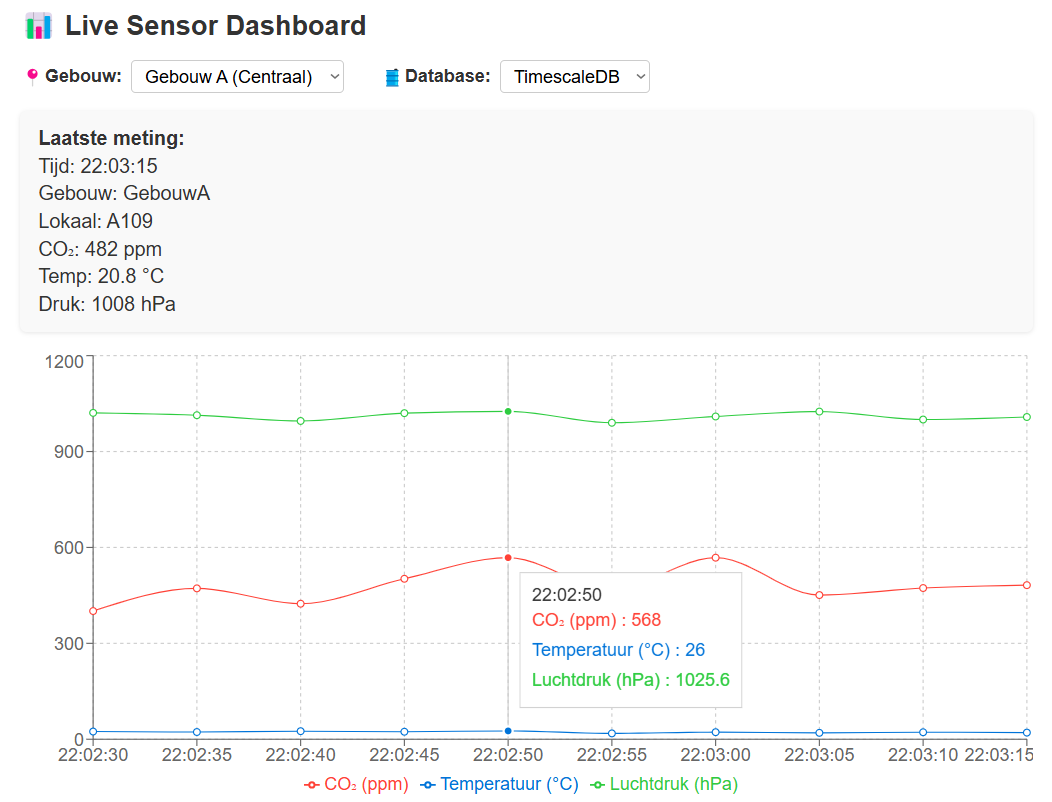
\includegraphics[width=0.8\textwidth]{GebouwA_TimeScale_Website.png}
	\caption{Frontendweergave met centrale database-architectuur (TimescaleDB, Gebouw A).}
    \label{fig:gebouw-a-architecture}
\end{figure}

\begin{figure}[H]
    \centering
    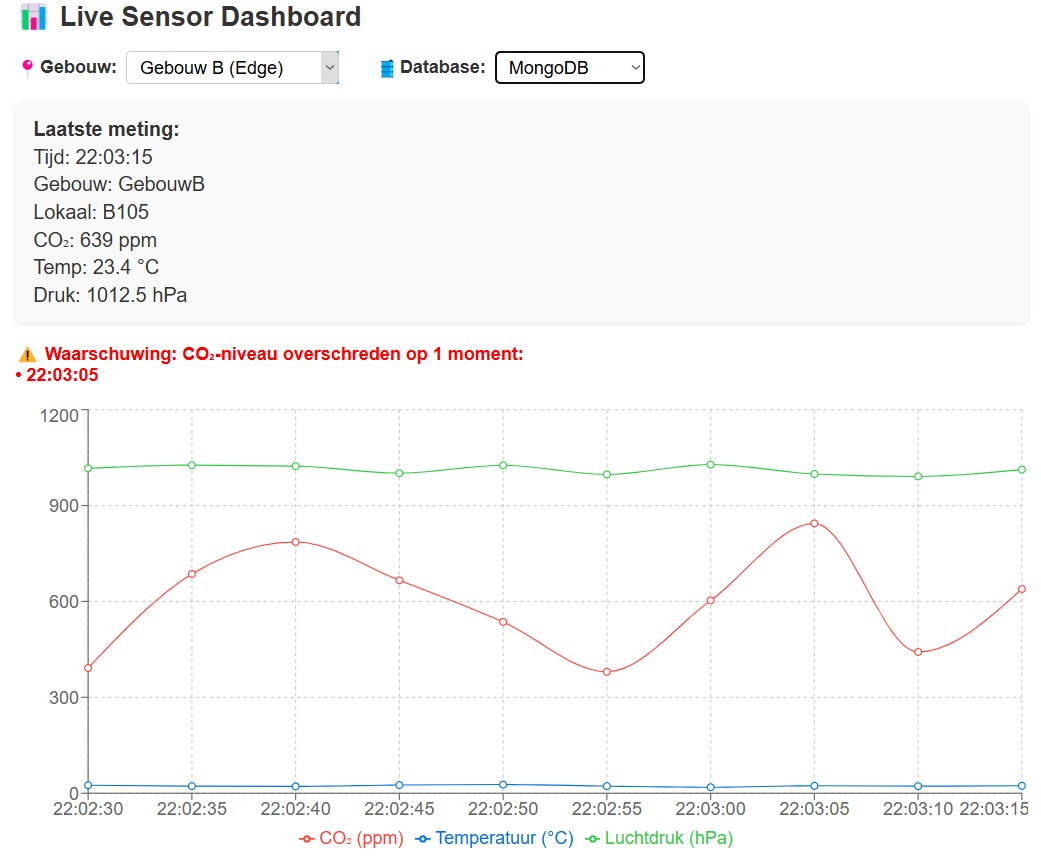
\includegraphics[width=0.8\textwidth]{GebouwB_MongoDb_Website.png}
    \caption{Frontendweergave met edge computing-architectuur (MongoDB, Gebouw B).}
    \label{fig:gebouw-b-architecture}
\end{figure}

De volledige code van het dashboard is beschikbaar via GitHub: \\
\href{https://github.com/WoutVC/bachelorproef2024/blob/main/proof_of_concept/frontend/src/components/LiveDashBoard.js}{LiveDashBoard.js}

\subsection{Resultaten en Grafieken}
De resultaten van de uitgevoerde tests met het script \href{https://github.com/WoutVC/bachelorproef2024/blob/main/proof_of_concept/backend/POCTests.js}{POCTests.js} zijn hieronder weergegeven in grafieken. Elke grafiek toont hoe de verschillende database-opstellingen presteren op vlak van snelheid, betrouwbaarheid en schaalbaarheid.

\begin{figure}[H]
	\centering
	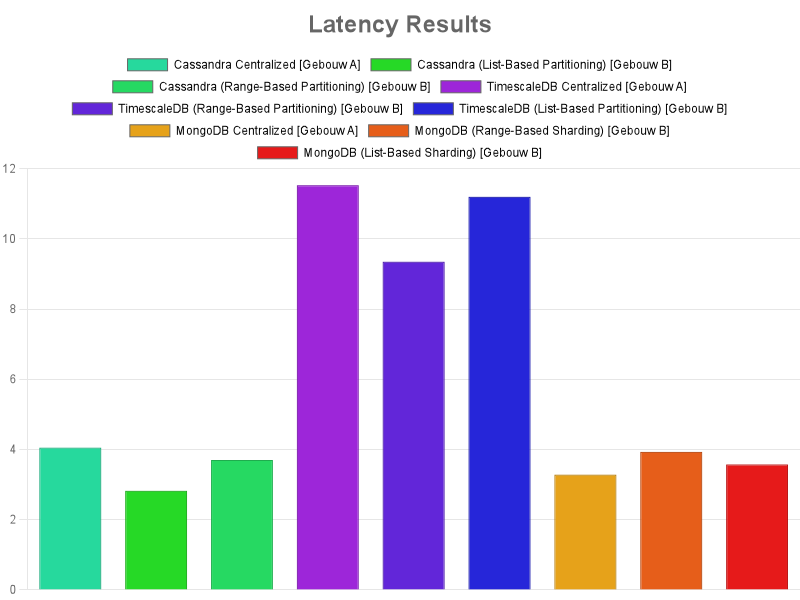
\includegraphics[width=0.8\textwidth]{Latency.png}
	\caption{Latentie van Cassandra, MongoDB en TimescaleDB (hoe snel data wordt gelezen).}
	\label{fig:latency-comparison}
\end{figure}

\paragraph{Hoe werd latentie getest?}
Latentie werd getest door 100 keer data op te vragen en te meten hoe lang dat gemiddeld duurde. Dit geeft aan hoe snel een database reageert op leesverzoeken.

\paragraph{Resultaat en analyse:}
\textit{Cassandra met list-partitionering} had de laagste latentie (2.82 ms), gevolgd door \textit{MongoDB met list-sharding} (3.57 ms). \textit{TimescaleDB met range-partitionering} was trager (9.35 ms). Dat betekent dat Cassandra en MongoDB iets beter zijn voor toepassingen waar snelheid belangrijk is.

\begin{figure}[H]
	\centering
	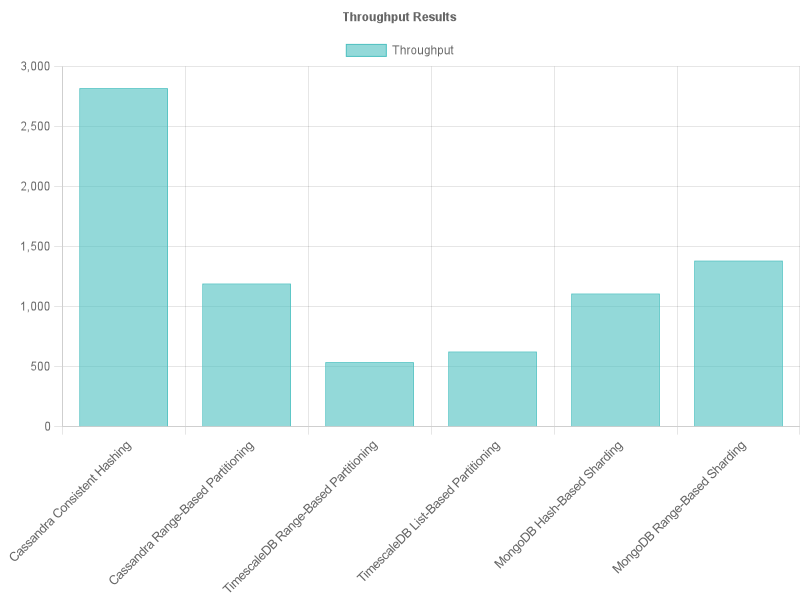
\includegraphics[width=0.8\textwidth]{Throughput.png}
	\caption{Throughput (hoeveel data per seconde) van de databases.}
	\label{fig:throughput-comparison}
\end{figure}

\paragraph{Hoe werd throughput getest?}
Hierbij werd 100 keer data opgeslagen in elke database. Daarna werd berekend hoeveel records per seconde verwerkt werden. Dit toont hoe snel een database kan schrijven.

\paragraph{Resultaat en analyse:}
De verschillen in throughput waren klein. \textit{TimescaleDB met list-partitionering} scoorde het best (4.86 records/s), gevolgd door \textit{TimescaleDB centraal} en \textit{MongoDB centraal}. Alle databases presteerden dus vrij goed en gelijkaardig op dit vlak.

\begin{figure}[H]
	\centering
	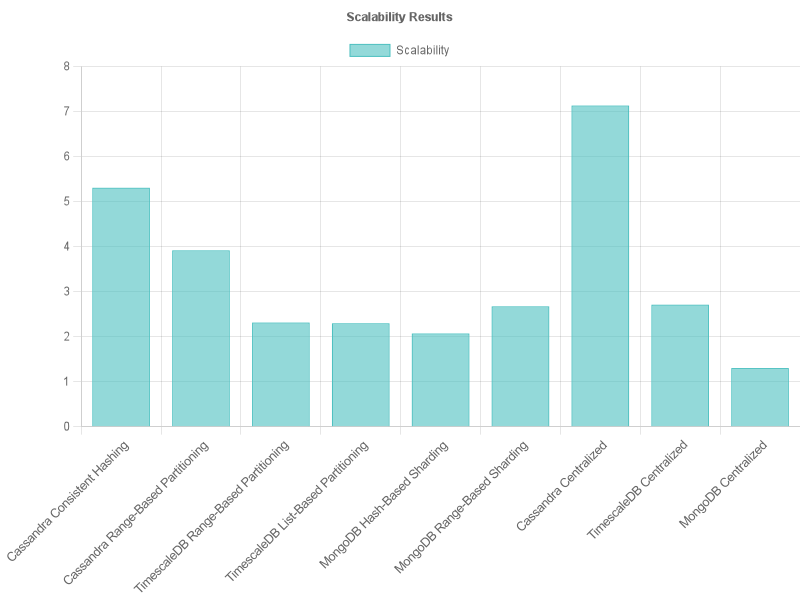
\includegraphics[width=0.8\textwidth]{Scalability.png}
	\caption{Schaalbaarheid (hoe goed presteren bij grotere hoeveelheden data).}
	\label{fig:scalability-comparison}
\end{figure}

\paragraph{Hoe werd schaalbaarheid getest?}
Het aantal records werd stapsgewijs verhoogd (10, 50, 100) en de verwerkingstijd werd gemeten. Hoe minder vertraging er optrad bij grote hoeveelheden data, hoe beter de schaalbaarheid.

\paragraph{Resultaat en analyse:}
\textit{TimescaleDB met range-partitionering} behaalde de hoogste score van 5,67. Ook \textit{Cassandra met list-partitionering} (4,79) en \textit{TimescaleDB centraal} (4,97) presteerden goed. \textit{MongoDB centraal} had met 1,95 de laagste score, wat duidt op minder goede schaalbaarheid bij grote datasets.

\subsection{Consistentie}
\begin{figure}[H]
\centering
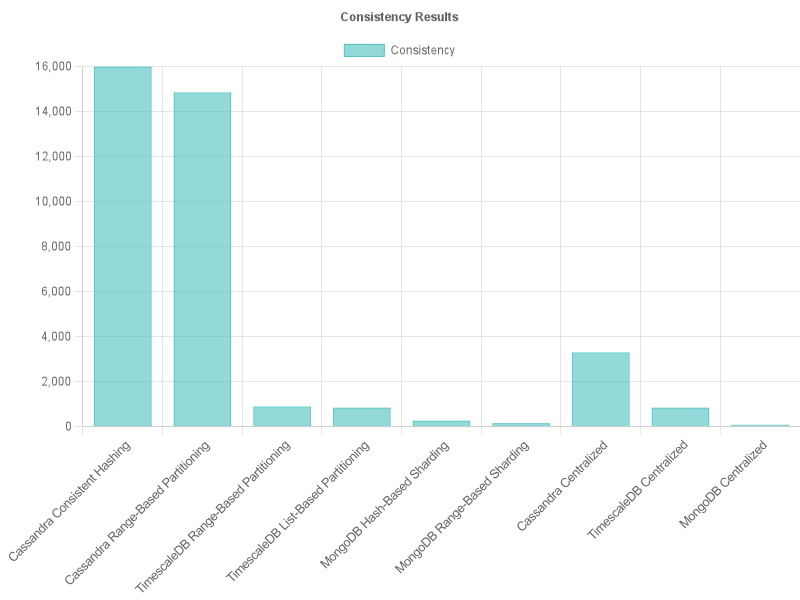
\includegraphics[width=0.8\textwidth]{Consistency.png}
\caption{Consistentie (hoe snel nieuwe data zichtbaar wordt voor gebruikers).}
\label{fig:consistency-comparison}
\end{figure}

\paragraph{Hoe werd consistentie getest?}
Nieuwe gegevens werden weggeschreven en onmiddellijk opgehaald. Het aantal direct beschikbare records werd gemeten. Een database waarbij data meteen zichtbaar is, wordt als consistent beschouwd.

\paragraph{Resultaat en analyse:}
Alle databases scoorden 10/10, wat betekent dat elke nieuwe record direct beschikbaar was.

\begin{figure}[H]
    \centering
    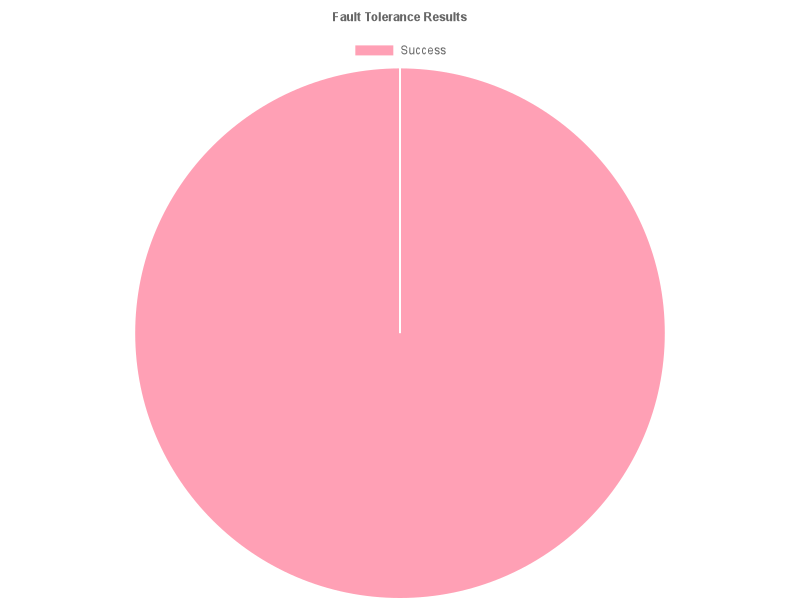
\includegraphics[width=0.8\textwidth]{Fault_Tolerance.png}
    \caption{Fouttolerantie (hoe goed een database omgaat met fouten of verbindingsproblemen).}
    \label{fig:fault-tolerance-comparison}
\end{figure}

\paragraph{Hoe werd fouttolerantie getest?}
Tijdens deze test werd de databaseverbinding tijdelijk onderbroken. Daarna werd getest of het systeem zich automatisch herstelde en correct verder werkte.

\paragraph{Resultaat en analyse:}
Alle databases haalden een score van 1.00. Ze konden dus allemaal goed herstellen van de fout en er ging geen data verloren. Dat is belangrijk in een echte IoT-omgeving waar netwerkproblemen kunnen voorkomen.

\subsection{Testresultaten en Tabeloverzicht}
Naast de grafieken biedt deze tabel een samenvatting van de testresultaten.

\begin{table}[h]
    \centering
    \resizebox{\textwidth}{!}{
    \begin{tabular}{|l|c|c|c|c|c|}
        \hline
        \textbf{Database}                                 & \textbf{Fault Tolerance} & \textbf{Scalability} & \textbf{Realtime Latency} & \textbf{Realtime Throughput} & \textbf{Consistency} \\ \hline
        Cassandra Centralized [Gebouw A]                  & 1                        & 3.74                 & 4.05                      & 4.78                         & 10                   \\ \hline
        Cassandra (List-Based Partitioning) [Gebouw B]   & 1                        & 4.79                 & 2.82                      & 4.78                         & 10                   \\ \hline
        Cassandra (Range-Based Partitioning) [Gebouw B]  & 1                        & 2.62                 & 3.70                      & 4.80                         & 10                   \\ \hline
        TimescaleDB Centralized [Gebouw A]                & 1                        & 4.97                 & 11.53                     & 4.83                         & 10                   \\ \hline
        TimescaleDB (Range-Based Partitioning) [Gebouw B] & 1                       & 5.67                 & 9.35                      & 4.82                         & 10                   \\ \hline
        TimescaleDB (List-Based Partitioning) [Gebouw B] & 1                        & 4.73                 & 11.20                     & 4.86                         & 10                   \\ \hline
        MongoDB Centralized [Gebouw A]                    & 1                        & 1.95                 & 3.28                      & 4.84                         & 10                   \\ \hline
        MongoDB (Range-Based Sharding) [Gebouw B]         & 1                       & 2.33                 & 3.93                      & 4.77                         & 10                   \\ \hline
        MongoDB (List-Based Sharding) [Gebouw B]          & 1                       & 2.04                 & 3.57                      & 4.78                         & 10                   \\ \hline
    \end{tabular}
    }
    \caption{Vergelijking van prestaties tussen Cassandra, MongoDB en TimescaleDB in centrale en edge (Gebouw B) configuraties.}
    \label{tab:test-results}
\end{table}

\subsection{Conclusie}
De evaluatie van de databases is gebaseerd op een gewogen scoresysteem (\href{https://github.com/WoutVC/bachelorproef2024/blob/main/proof_of_concept/backend/analyzeResults.js}{analyzeResults.js}), waarbij de volgende stappen worden uitgevoerd:

\paragraph{Consolidatie van resultaten:} 
Voor elke database worden de resultaten per meetwaarde samengevoegd. Voor meetwaarden zoals schaalbaarheid (Scalability) en fouttolerantie (Fault Tolerance), waarvoor meerdere metingen beschikbaar zijn, wordt het gemiddelde berekend.

\paragraph{Normalisatie van scores:} 
De numerieke scores voor elke meetwaarde worden genormaliseerd naar een schaal van 0 tot 1 op basis van het minimum en maximum onder alle databases:
\[
\text{Genormaliseerde score} = \frac{\text{Waarde} - \text{Minimum}}{\text{Maximum} - \text{Minimum}}
\]
Indien minimum en maximum gelijk zijn, wordt een neutrale score toegekend (bijvoorbeeld 0.5).

Voor meetwaarden waarbij een hogere score beter is (zoals throughput, schaalbaarheid, fouttolerantie en consistentie) wordt deze genormaliseerde score direct gebruikt. Voor meetwaarden waarbij een lagere score beter is (zoals latentie) wordt de genormaliseerde score omgekeerd berekend, zodat een lagere oorspronkelijke waarde leidt tot een hogere genormaliseerde score.

\paragraph{Gewogen totaalscore:} 
De genormaliseerde scores worden vervolgens gewogen op basis van vooraf bepaalde belangrijkheidsfactoren per meetwaarde en opgeteld tot een totaalscore per database.


\textbf{Toepassing van gewichten:} Elke meetwaarde krijgt een gewicht op basis van het relatieve belang voor edge computing. De toegepaste gewichten zijn als volgt:
\begin{itemize} 
	\item \textbf{Fouttolerantie - 20\% (Must Have):}  
	De apparaten aan de rand van het netwerk moeten goed blijven werken, zelfs bij tijdelijke stroom- of netwerkproblemen. Gegevens mogen niet verloren gaan.

	\item \textbf{Schaalbaarheid - 20\% (Should Have):}  
	Aangezien er mogelijk honderden lokalen zijn, moet het systeem makkelijk groter gemaakt kunnen worden zonder dat het trager wordt.

	\item \textbf{Verwerkingssnelheid - 15\% (Should Have):}  
	Het systeem moet snel genoeg zijn om alle gegevens van de sensoren op tijd te verwerken.

	\item \textbf{Latentie - 15\% (Should Have):}  
	De vertraging tussen het meten van gegevens en het verwerken of opslaan ervan moet zo klein mogelijk zijn om real-time inzichten mogelijk te maken.

	\item \textbf{Gegevensconsistentie - 10\% (Could Have):}  
	Het is minder erg als data niet altijd 100 \% gelijk is op alle plaatsen, zolang het systeem maar snel en beschikbaar blijft. Toch is het belangrijk bij het samenvoegen van meetgegevens.
\end{itemize}

\paragraph{Berekening van totaalscores:} 
Om de verschillende databases goed met elkaar te kunnen vergelijken, werd voor elke database een totaalscore berekend. Deze score is gebaseerd op een combinatie van vijf belangrijke eigenschappen: fouttolerantie, schaalbaarheid, latency (vertraging), throughput (verwerkingssnelheid) en consistentie. Hoe beter een database scoorde op deze eigenschappen, hoe hoger haar totaalscore. Lagere latency werd hierbij als beter beschouwd. Alle scores zijn genormaliseerd zodat ze eerlijk met elkaar vergeleken kunnen worden.

\paragraph{Totaalscores en rangschikking:}

Op basis van deze berekening ziet de top 3 er als volgt uit:

\begin{itemize}
    \item \textbf{TimescaleDB (Range-Based Partitioning) [Gebouw B]} Score: \textbf{7.76}  
    Deze configuratie scoorde het best. Vooral op het vlak van schaalbaarheid en snelheid presteert deze database zeer goed, wat ze ideaal maakt voor realtime toepassingen in een edge-omgeving.

    \item \textbf{Cassandra (List-Based Partitioning) [Gebouw B]} Score: \textbf{7.74}  
    Cassandra met list-based partitioning presteerde het beste op vlak van latency. Dankzij zijn combinatie van snelheid, fouttolerantie en goede prestaties is dit een sterke keuze voor realtime monitoring aan de rand van het netwerk.

    \item \textbf{TimescaleDB (List-Based Partitioning) [Gebouw B]} Score: \textbf{7.56}  
    Deze configuratie scoort vooral goed op throughput en is een stabiele keuze voor systemen die continu veel data moeten verwerken, zoals dashboards of IoT-systemen.
\end{itemize}

\paragraph{Conclusie:}
De testresultaten tonen aan dat databases in de edge-omgeving (Gebouw B) met een goede partitionering beter presteren dan gecentraliseerde databases.  
Binnen de context van de HoGent-use case blijkt \textbf{TimescaleDB met range-based partitioning} de meest geschikte keuze. Deze database biedt een goede balans tussen schaalbaarheid, snelheid en betrouwbaarheid, wat belangrijke eigenschappen zijn voor een systeem dat voortdurend grote hoeveelheden sensordata moet verwerken.